\chapter{Preliminary Graph Theory}\label{ch:prelim}

First, let's define some basic concepts of graph theory, starting with the graph itself.

\section{Graphs}

\begin{definition}
    A graph is an algebraic structure most commonly used to describe relationships between objects. There are many definitions of a graph. The most abstract deefinition of a graph is simply a set $V$ and a relation $R$ on $V$ denoting which elements of $V$ are connected. Graphs in general are \textit{directed}, if $R$ is symmetric, the graph is \textit{undirected}. For the purposes of this work we will be using a geometric definition and generally undirected graphs. An undirected graph is an ordered pair $G = (V, E)$, where $V$ is a set of \textit{vertices} and $E$ is a set of edges, i. e. a set of unordered pairs of vertices $\forall e \in E: ~ e = (u,v); u,v \in V$.
\end{definition}

\begin{figure}[h]
    \centering
        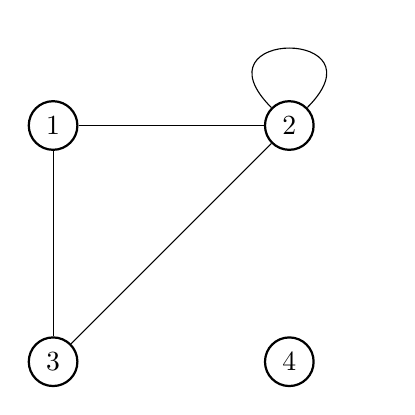
\begin{tikzpicture}
            \begin{scope}[every node/.style={circle,thick,draw}]
                \node (1) at (0,0) {1};
                \node (2) at (3,0) {2};
                \node (3) at (0,-3) {3};
                \node (4) at (3,-3) {4};
            \end{scope}
            \begin{scope}[every loop/.style={}]
                \path
                    (1) edge (2)
                    (2) edge (3)
                    (3) edge (1)
                    (2) edge [loop] (2);
            \end{scope}
        \end{tikzpicture}
\end{figure}

\begin{definition}
    A \textit{path} in a graph $G$ from $v$ to $w$; $v,w \in V$ is a sequence of vertices $(u_1, u_2, \dots, u_n); ~ \{u_i ~|~ 1 \leq i \leq n\} \subseteq V$ such that $u_1 = v$, $u_n = w$ and $\{(u_i, u_{i+1}) ~|~ 1 \leq i \leq n-1\} \subseteq E$.
\end{definition}

\begin{definition}
    A graph is \textit{connected} if there exists a path between every pair of vertices $v,w \in V; ~ v \neq w$.
\end{definition}

The example provided above is not connected as the vertex $4$ is isolated. Below is an example of a similar graph that is connected.

\begin{figure}[h]
    \centering
        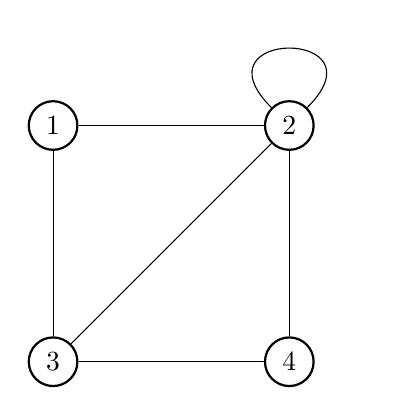
\begin{tikzpicture}
            \begin{scope}[every node/.style={circle,thick,draw}]
                \node (1) at (0,0) {1};
                \node (2) at (3,0) {2};
                \node (3) at (0,-3) {3};
                \node (4) at (3,-3) {4};
            \end{scope}
            \begin{scope}[every loop/.style={}]
                \path
                    (1) edge (2)
                    (2) edge (3)
                    (3) edge (1)
                    (2) edge [loop] (2)
                    (2) edge (4)
                    (3) edge (4);
            \end{scope}
        \end{tikzpicture}
\end{figure}

\begin{definition}
    A \textit{degree} $\Delta (v)$ of a vertex $v$ denotes how many edges are incident to this vertex.
\end{definition}

\begin{definition}
    A graph is \textit{k-regular} if the degree of each vertex is $k$. A \textit{cubic graph} is a 3-regular graph.
\end{definition}

As an example, the $K_4$ graph is cubic.

\begin{figure}[h]
    \centering
        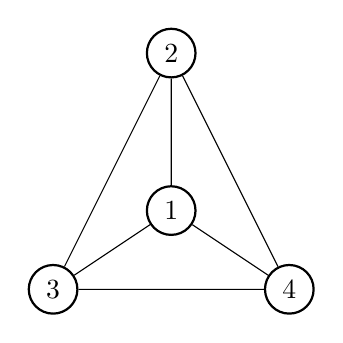
\begin{tikzpicture}
            \begin{scope}[every node/.style={circle,thick,draw}]
                \node (1) at (0,0) {1};
                \node (2) at (0,2) {2};
                \node (3) at (-1.5,-1) {3};
                \node (4) at (1.5,-1) {4};
            \end{scope}
            \draw (1) -- (2) -- (3) -- (4) -- (1) (2) -- (4) (1) -- (3);
        \end{tikzpicture}
\end{figure}

In general statements about graphs in later chapters, we are referring to unordered cubic graphs.

\subsection{Coloring}

When simple binary relationships between objects are not enough, graphs can be used to "quantify" these relationships. The edges of a graph can be assigned weights, leading us to fields like nowhere-zero flows and edge colorings.

\begin{definition}
    An \textit{edge coloring} $\gamma : E(G) \rightarrow C$ of a graph $G$ assigns to each edge of $G$ one color from a set of colors $C$. A \textit{proper} coloring has each color present at each vertex at most once.

    $$(\forall u \in V)(\forall v,w \in V; (u,v) \in E(G) \land (u,w) \in E(G)) ~ \gamma((u,v)) \neq \gamma((u,w))$$

    A proper coloring using $k$ colors is called a \textit{k-coloring}
\end{definition}

Although colors are a nice visualization of a coloring, the colors are not implied in the literal sense. Instead the color set $C$ is usually a subset of $\mathbb{N}$.

The canonical coloring problem is to find the minimum number of colors required for a proper coloring. This number is called the \textit{chromatic number} for vertex colorings and \textit{chromatic index} for edge colorings. Determining the chromatic number and index is useful in other areas of graph theory as well.

\begin{theorem}\label{th:bipartite}
    A graph is bipartite if and only if it has a proper vertex 2-coloring.
\end{theorem}

\begin{theorem}[Vizing]
    The chromatic index of a graph $G$ is $\Delta(G)$ or $\Delta(G) + 1$.
\end{theorem}

In other words, we can always color the edges of a graph using at most $\Delta(G) + 1$ colors where $\Delta(G)$ is the highest degree of any vertex in $G$. The lower bound $\Delta(G)$ is trivial; we need exactly $\Delta(G)$ colors at the highest degree vertex in $G$ to construct a proper coloring. The Vizing theorem\todo{CITE VIZING THEOREM} proves the upper bound using Kempe chains.

\section{Signed graphs}

A signed graph is a graph in which each edge has either a positive or a negative sign. There are multiple definitions of a signed graph but for our purposes a sign function is most practical.

\begin{definition}
    A \textit{signed graph} $\Gamma = (G, \sigma)$ consists of a \textit{base graph} $G$ and a \textit{sign function} $\sigma : E(G) \rightarrow \{+,-\}$ that assigns a sign to each edge of $G$.
\end{definition}

Below is an example of a signed graph.

\begin{figure}[h]
    \centering
        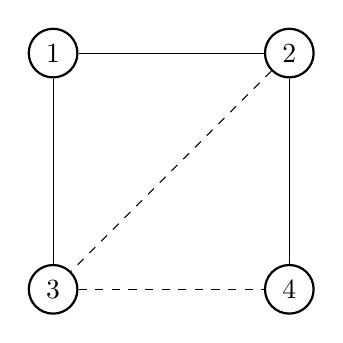
\begin{tikzpicture}
            \begin{scope}[every node/.style={circle,thick,draw}]
                \node (1) at (0,0) {1};
                \node (2) at (3,0) {2};
                \node (3) at (0,-3) {3};
                \node (4) at (3,-3) {4};
            \end{scope}
            \begin{scope}[every loop/.style={}]
                \path
                    (1) edge (2)
                    (2) edge [dashed] (3)
                    (3) edge (1)
                    (2) edge (4)
                    (3) edge [dashed] (4);
            \end{scope}
        \end{tikzpicture}
\end{figure}

A fundamental concept in the signed graphs theory is \textit{balance}. The sign of a path is the product of the signs of its edges. A path is positive if and only if there is an even number of negative edges on it. A cycle is balanced if it is positive and a signed graph is balanced if each cycle in it is balanced\cite{harary}.

\begin{theorem}[Harary]\label{th:harary}
    A signed graph is balanced if
    \begin{enumerate}
        \item for every pair of vertices, all paths between these vertices is positive
        \item the vertices can be divided into two subsets (possibly empty) such that each edge with both ends in the same subset is positive and each edge with ends in different subsets is negative
    \end{enumerate}

    This is the generalization of the bipartite graph theorem.\cref{th:bipartite}
\end{theorem}

The proof uses the method of \textit{switching}. Switching a vertex of a signed graph reverses the sign of each edge incident to it. More generally, switching a signed graph reverses the sign of each edge between a vertex subset and its complement.

\begin{figure}[h]\label{fig:switching}
    \centering
        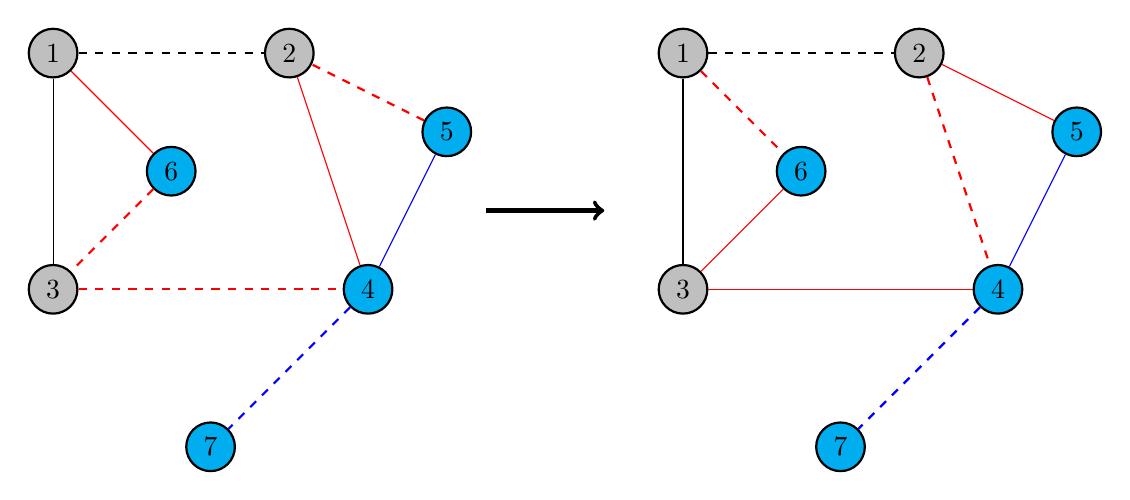
\begin{tikzpicture}
            \begin{scope}[every node/.style={circle,thick,draw,fill=lightgray}]
                \node (1) at (0,0) {1};
                \node (2) at (3,0) {2};
                \node (3) at (0,-3) {3};
            \end{scope}
            \begin{scope}[every node/.style={circle,thick,draw,fill=cyan}]
                \node (4) at (4,-3) {4};
                \node (5) at (5,-1) {5};
                \node (6) at (1.5,-1.5) {6};
                \node (7) at (2,-5) {7};
            \end{scope}
            \begin{scope}[every edge/.style={draw,dashed,thick}]
                \path
                    (1) edge (2)
                    (3) edge [color=red] (4)
                    (4) edge [color=blue] (7)
                    (5) edge [color=red] (2)
                    (6) edge [color=red] (3);
            \end{scope}
            \begin{scope}[every every edge/.style={draw,thick}]
                \path
                    (1) edge [color=red] (6)
                    (3) edge (1)
                    (4) edge [color=blue] (5)
                    (2) edge [color=red] (4);
            \end{scope}

            \draw [ultra thick, ->] (5.5,-2) -- (7,-2);

            \begin{scope}[every node/.style={circle,thick,draw,fill=lightgray}]
                \node (11) at (8,0) {1};
                \node (21) at (11,0) {2};
                \node (31) at (8,-3) {3};
            \end{scope}
            \begin{scope}[every node/.style={circle,thick,draw,fill=cyan}]
                \node (41) at (12,-3) {4};
                \node (51) at (13,-1) {5};
                \node (61) at (9.5,-1.5) {6};
                \node (71) at (10,-5) {7};
            \end{scope}
            \begin{scope}[every edge/.style={draw,dashed,thick}]
                \path
                    (21) edge [color=red] (41)
                    (11) edge [color=red] (61)
                    (11) edge (21)
                    (41) edge [color=blue] (71);
            \end{scope}
            \begin{scope}[every every edge/.style={draw,thick}]
                \path
                    (31) edge (11)
                    (41) edge [color=blue] (51)
                    (31) edge [color=red] (41)
                    (51) edge [color=red] (21)
                    (61) edge [color=red] (31);
            \end{scope}
        \end{tikzpicture}
    \caption[Example of a switching]{Example of a switching. Note that switching blue vertices and switching grey vertices results in the same transformation.}
\end{figure}

We can prove by induction that a signed graph can be switched to an all-positive graph if and only if it is balanced.

\begin{definition}
    If a signed graph can be obtained from another signed graph by switching, they are considered \textit{equivalent}. For a single base graph, switching forms \textit{equivalence classes} of signed graphs; within a single equivalence class all graphs can be switched to each other.
\end{definition}

It makes sense to study properties of signed graphs that behave consistently under switching. An example of such property is the sign of cycles. Switching a single vertex doesn't change the sign of cycles (cycles containing the vertex reverse signs for two edges resulting in the same product) and switching a set of vertices is equivalent to a sequence of one-vertex-switches (each edge within the set and within the complement gets reversed twice).

\subsection{Coloring}

\todo{}

\section{Motivation}

\say{In the study of various important and difficult problems in graph theory (such as the cycle double cover conjecture and the 5-flow conjecture), one encounters an interesting but somewhat mysterious variety of graphs called snarks. In spite of their simple definition [\dots] and over a century long investigation, their properties and structure are largely unknown.} --- Chladný, Škoviera \cite{skoviera-citat}

\todo{}
